\documentclass[a4paper,11pt]{article}
\usepackage[a4paper, margin=1.68cm, top=2cm]{geometry}
\usepackage{amssymb,amsmath}
\usepackage[pdftex]{graphicx}
\usepackage{float}
\usepackage{caption}
\captionsetup{justification=raggedright,singlelinecheck=false}
\usepackage{multirow}
\usepackage[table,xcdraw]{xcolor}
\usepackage{hyperref}
\usepackage{pdfpages}
\usepackage{fancyhdr}
\pagestyle{fancyplain}
\renewcommand{\headrulewidth}{0pt}
\DeclareMathOperator{\E}{\mathbb{E}}
\rhead{22nd March, 2018}
\lhead{King Fung Wong}

\graphicspath{ {/Users/kingf.wong/PycharmProjects/test/Risk Analysis Q1/} }

\begin{document}
\begin{flushleft}




\section{Task 1}
\begin{itemize}
\item[1.] After multiplying the number of holdings (positive for long positions and negative for short positions) to the historical stock prices and summing up the first log difference, the historical portfolio daily log-returns of the period Jan 1st, 2012 to 9th of February 2018 were obtained. The histogram of the return series, quantile-quantile plot, autocorrelation function of return, autocorrelation function of squared return are presented in the below figure. 


\begin{figure}[H]
\centerline{
  \begin{tabular}{@{}cccc@{}}
    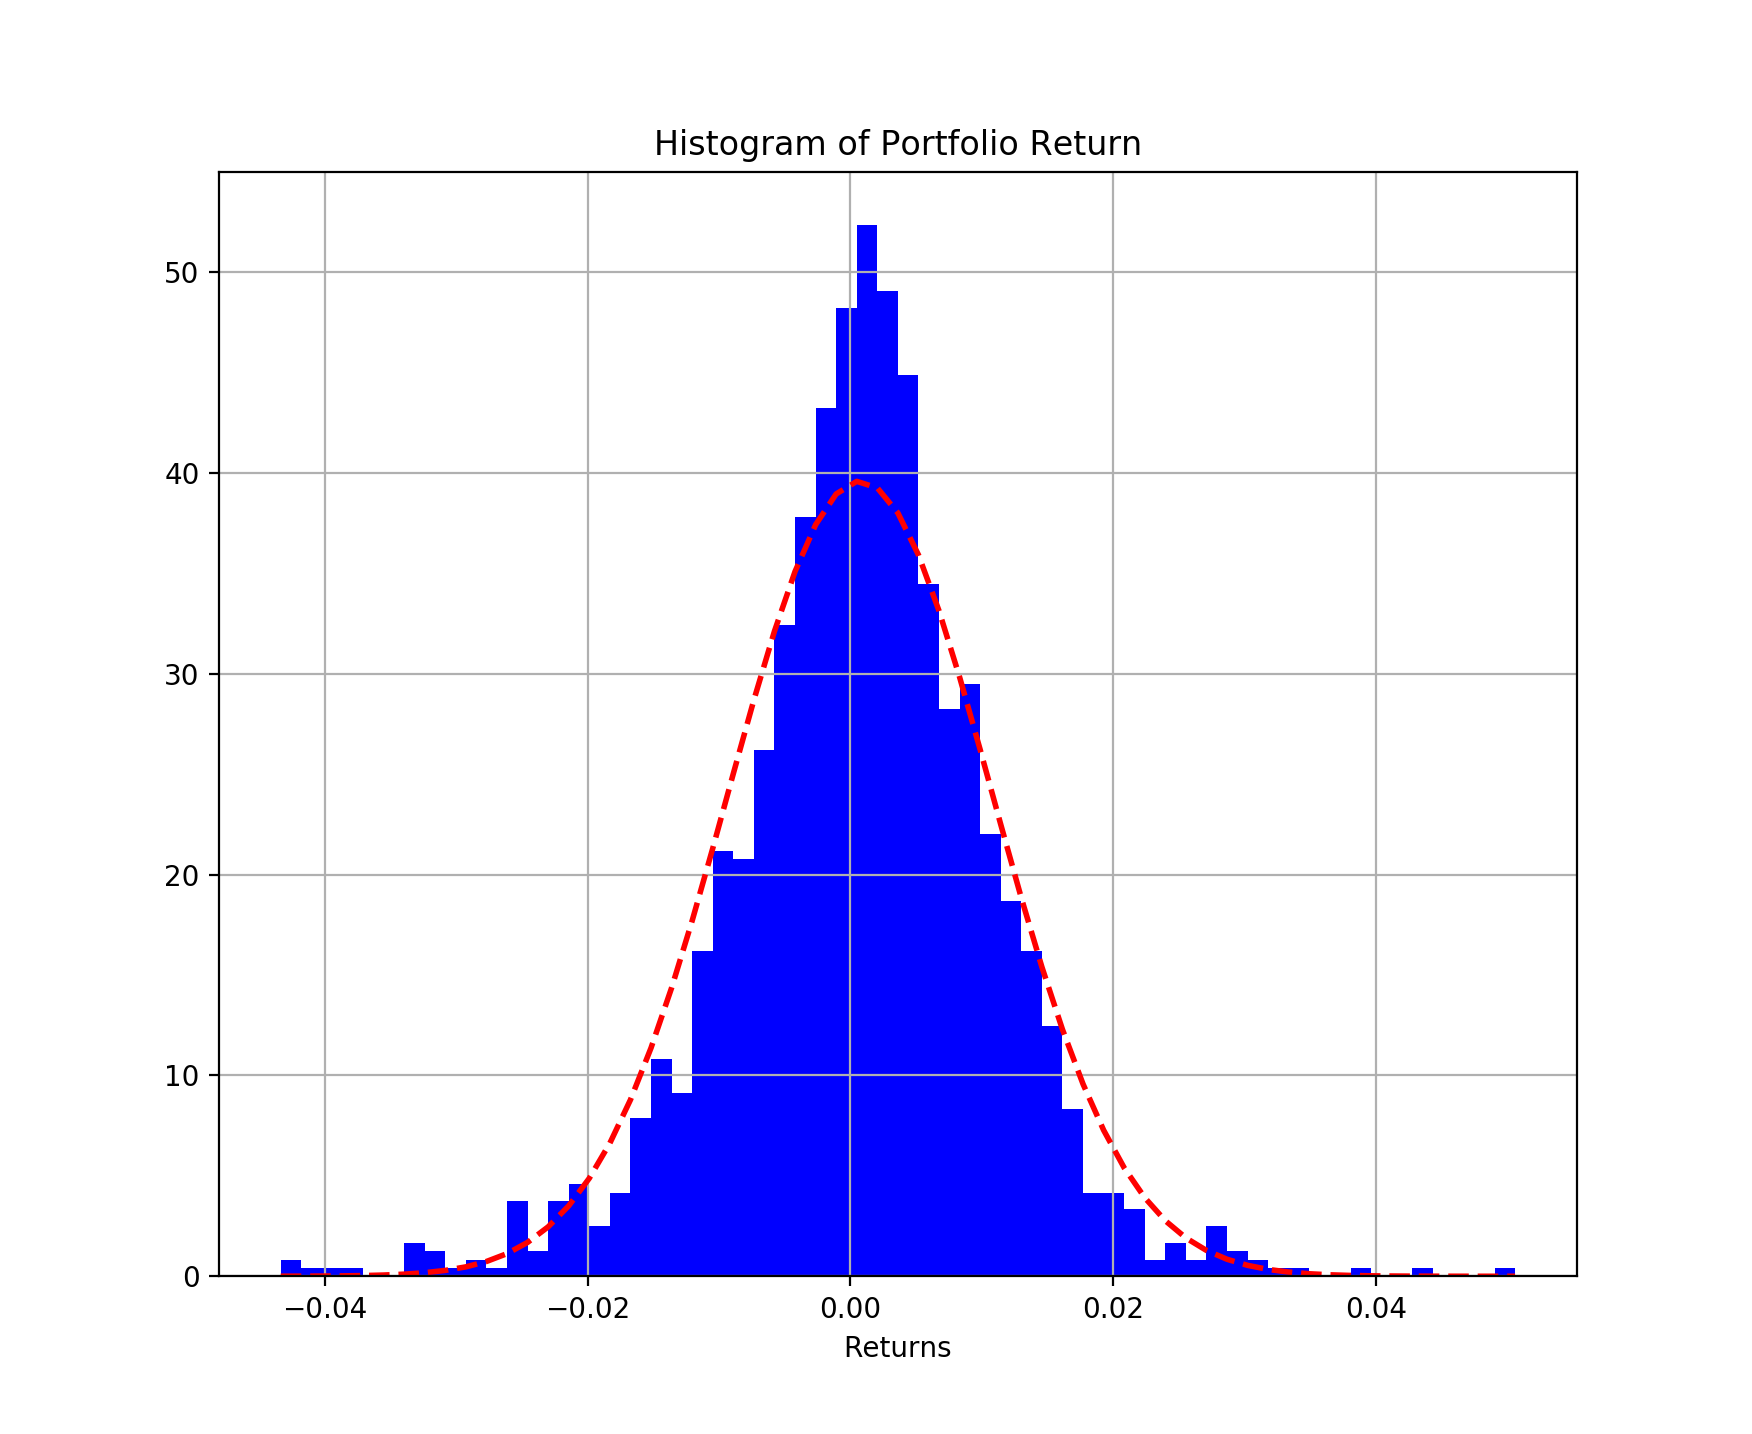
\includegraphics[scale=0.35]{hist_return.png} &
    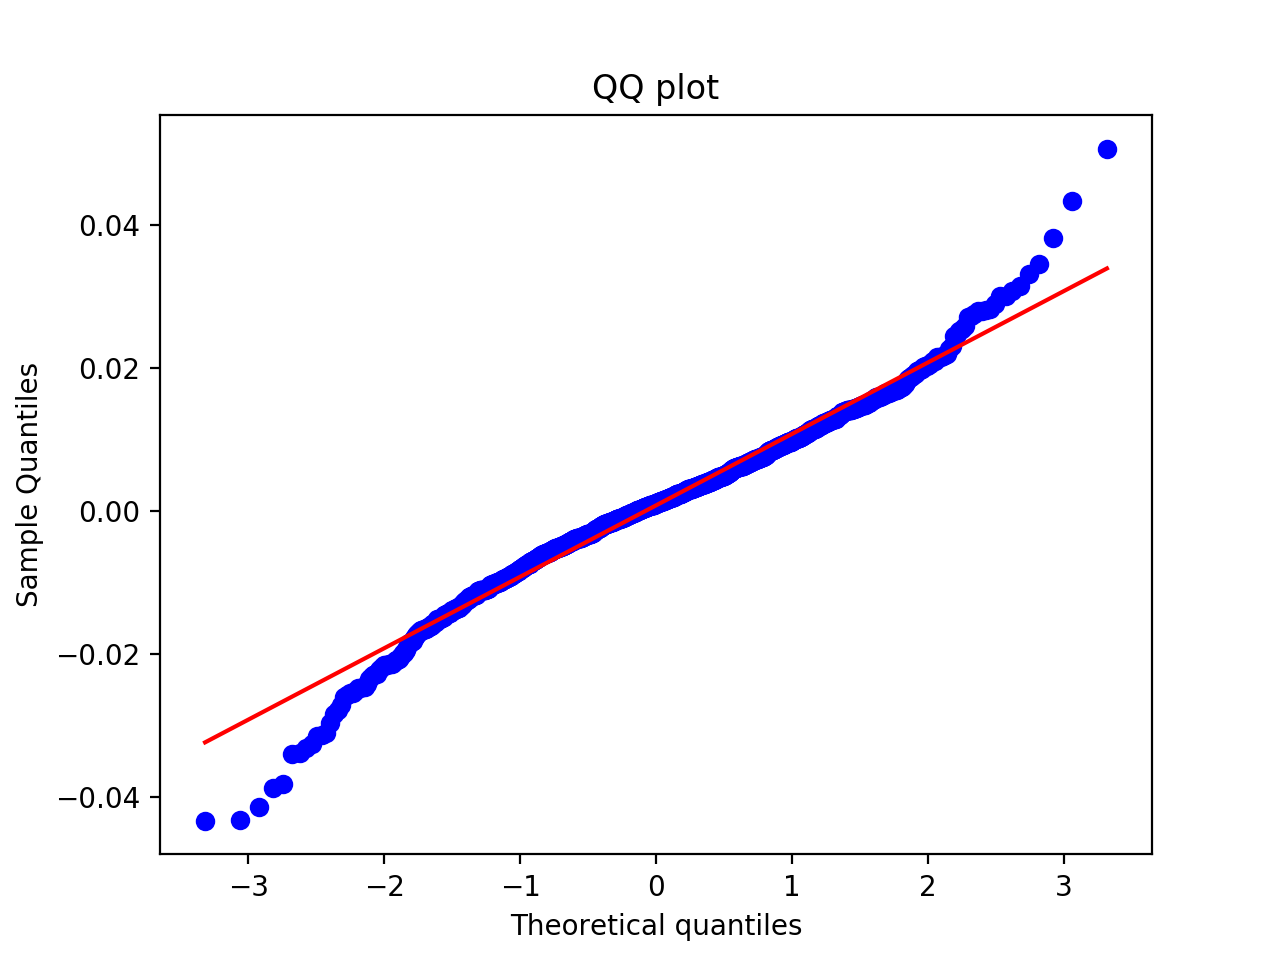
\includegraphics[scale=0.5]{ret_QQplot.png} \\
    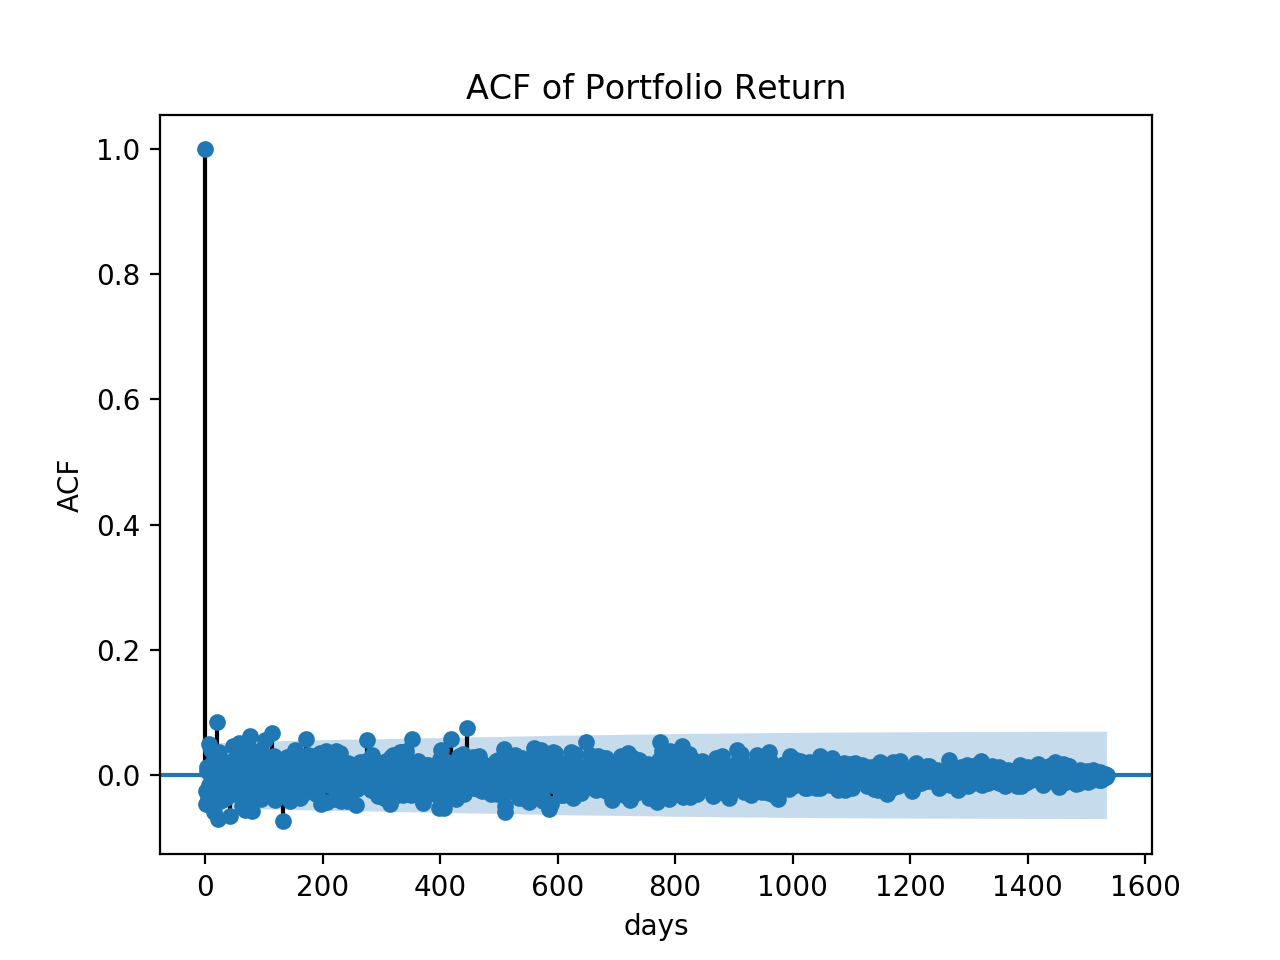
\includegraphics[scale=0.5]{ret_ACF.png} &
    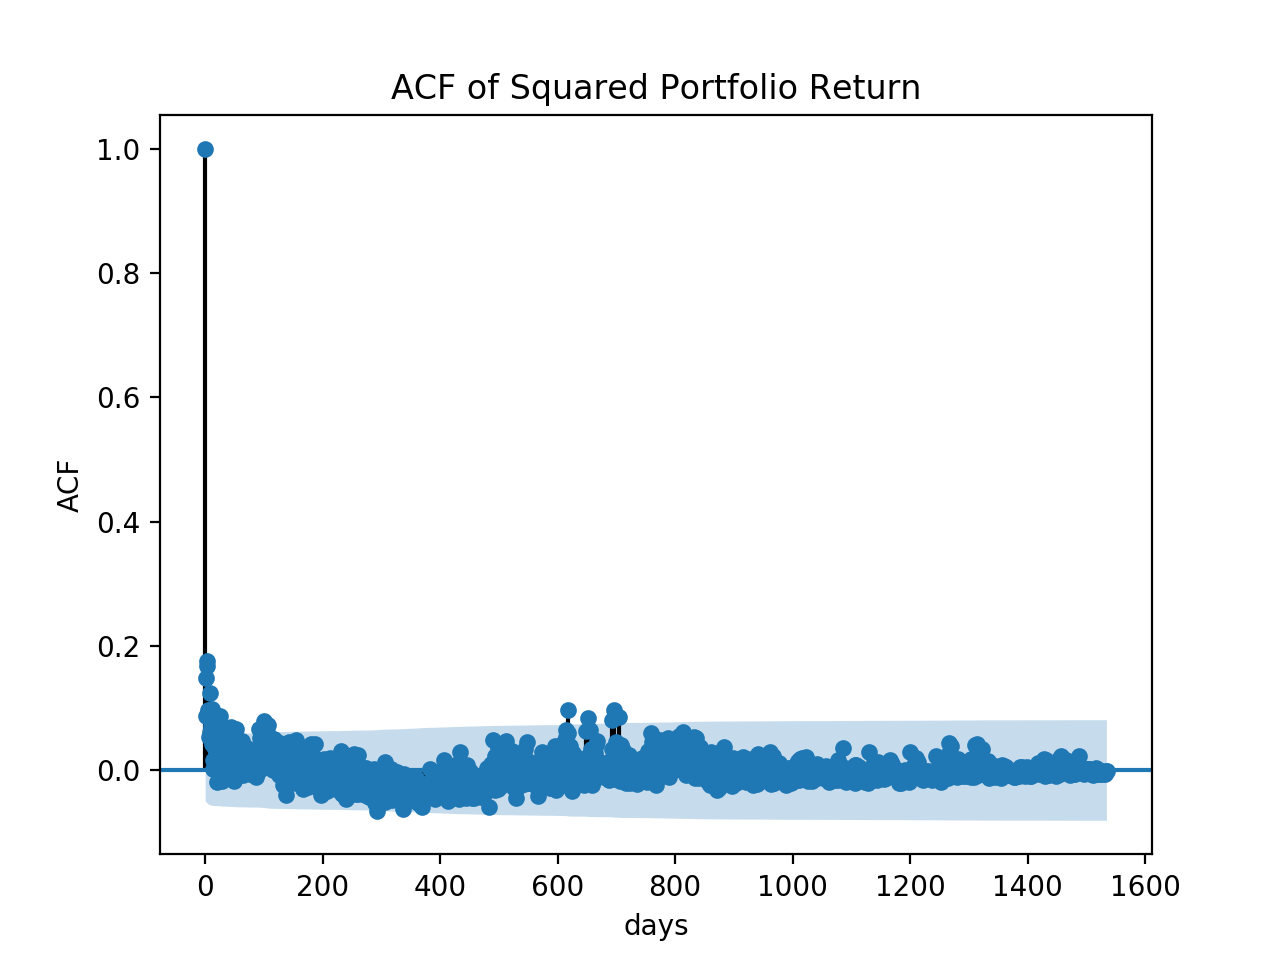
\includegraphics[scale=0.5]{sq_ret_ACF.png}   \\
  \end{tabular}}
  \caption{Top Left. Histogram fitted with the normal distribution in red Top Right. QQ plot Bottom Left ACF of the portfolio return Bottom Right ACF of the squared returns }
\end{figure}

The histogram shows the return distribution posses fatter tails than normal, excess kurtosis. The QQ plot shows the series is deviated from normal, indicated by the red line. The deviations on the top and bottom show the series has heavy tails and negatively skewed. The ACF plots shows the return series and squared return is highly autocorrelated with its first lag, deducing the returns and its variance are highly serially correlated with its first lagged value. 

The $Jarque \ and \ Bera$ statistic tests if the return series fits the normal distribution skewness and kurtosis. It is computed as follow

\begin{align*}
JB & = \frac{n-k+1}{6}\left(S^2+ \frac{1}{4} \left(C-3\right)^2\right),\\
\end{align*}
where
\begin{align*}
S &= \frac{\frac{1}{n}\sum_{i=1}^n\left(x_i - \bar{x}\right)^3}{\left(\frac{1}{n}\sum_{i=1}^n\left(x_i - \bar{x}\right)^2\right)^{3/2}} ,
C = \frac{\frac{1}{n}\sum_{i=1}^n\left(x_i - \bar{x}\right)^4}{\left(\frac{1}{n}\sum_{i=1}^n\left(x_i - \bar{x}\right)^2\right)^{2}}
\end{align*}

The Variance Ratio test tests if the the variance of the series equals to the  variance of the cumulative series. . If the square-root rule hold, the variance ratio should be closed to one and we do not reject the series is autocorrelated. We here set n = 30 days, 250 days. The z statistic is computed as follow $H_0  : \frac{\hat{\sigma}^2_{cum}}{n \hat{\sigma}^2} = \hat{VR(n)} = 1 $
\begin{align}
z\left(n\right) & = \frac{\hat{VR\left(n\right)}-1}{\sqrt{\frac{2\left(n-1\right)}{Tn}}} \sim \mathcal{N} \left(0,1\right),
\end{align}

\begin{table}[H]
\centerline{
\begin{tabular}{lllll}
\hline
\multicolumn{1}{c}{}           & \multicolumn{1}{c}{min}      & \multicolumn{1}{c}{max}     & \multicolumn{1}{c}{mean}      & \multicolumn{1}{c}{variance}  \\ \hline
\multicolumn{1}{c}{statistics} & \multicolumn{1}{c}{-0.04337} & \multicolumn{1}{c}{0.05060} & \multicolumn{1}{c}{0.0007363} & \multicolumn{1}{c}{0.0001015} \\ \hline
                               & skewness                     & excess-kurtosis             & Jarque Bera                   & $z_{\hat{VR}}$           \\ \hline
statistics                     & -0.2197                      & 1.9303                      & 250.8435 (0.0)                & -0.5757, -0.978                \\ \hline
\end{tabular}
}
\caption{Descriptive statistics of the portfolio returns}
\end{table}
The statistics above confirmed the return is negatively skewed and excess kurtosis. We rejected the null hypothesis that the return and squared returns are normally distributed according to their Jarque Bera statistic and p-value of zero. However the JB test should work with large enough number of sample ( $>$ 2000) where the portfolio series was only consist of 1536 returns. We do not reject the null hypothesis of zero-autocorrelation as the variance ratio test z score lies within the range of $-1.96 < z < 1.96$.


%\subsection{}
%\subsubsection{Gaussien daily VaR and Expected Shortfall}
\item[2.1] A foward rolling look back window of 250 days was created starting from July 1st 2014 and ending on Feb 9th 2018. The standard deviation of the portfolio returns in the look back window was calculated. The Gauss return forecast VaR, $VAR_{\alpha}$ was calculated as $\sigma z_{1-\alpha}$ where $\alpha$ was the confidence interval, 0.90 or 0.99. The expected shortfall was calculated as $\E\left(r_{ti} | r_{ti} < -VAR_{t\alpha}\right)$, the conditional mean of the simulated returns which were lower than the current forecast VaR. 
Using the scaling property of the Gaussian distribution. The $\sigma$ was scaled by $\sqrt(10/250)$ to give n-period VaR and n-period ES. 

%\subsubsection{Historical Simulation Bootstrap daily VaR and Expected Shortfall}
\item[2.2] The same rolling look back window was used for bootstrapping returns. The historical returns were randomly selected with replacement for 250 times (the number of samples available) to construct the simulated the daily PnL distribution. The $1-\alpha$ percentile was chose to be the simulated VaR with linear interpolation. The process was repeated for 2000 times ( could run 5000 times but doubling the computational time)  and the mean of simulated VaR was taken as the forecast VaR. The expected shortfall was calculated the same way as in Gauss ES. The mean of the simulated returns which were lower than the current simulated VaR was taken as one simulated ES. The procedure was repeated for 2000x and the mean of the simulated ES would be the forecast ES.

Calculating n-period VaR and ES requires simulating n-period returns from historical returns. The historical returns were randomly picked with replacment n x T times where T = 250 to construct n-period PnL distribution. The $1-\alpha$ percentile with linear interpolation was chose to be the simulated VaR and the average of the returns below simulated VaR would be the simulated ES. The process was repeated 2000 times to give one n-period forecast VaR and one n-period forecast ES. \\
The rolling forecast of return VaR and ES of each model were overlaid on the historical portfolio returns. The green lines represent violation of VaR and the red lines represent the number of violations of Expected Shortfall in each model backtesting from Jan 1st, 2012 to 9th of February 2018. 
\begin{figure}[H]
\centerline{
  \begin{tabular}{@{}cccc@{}}
    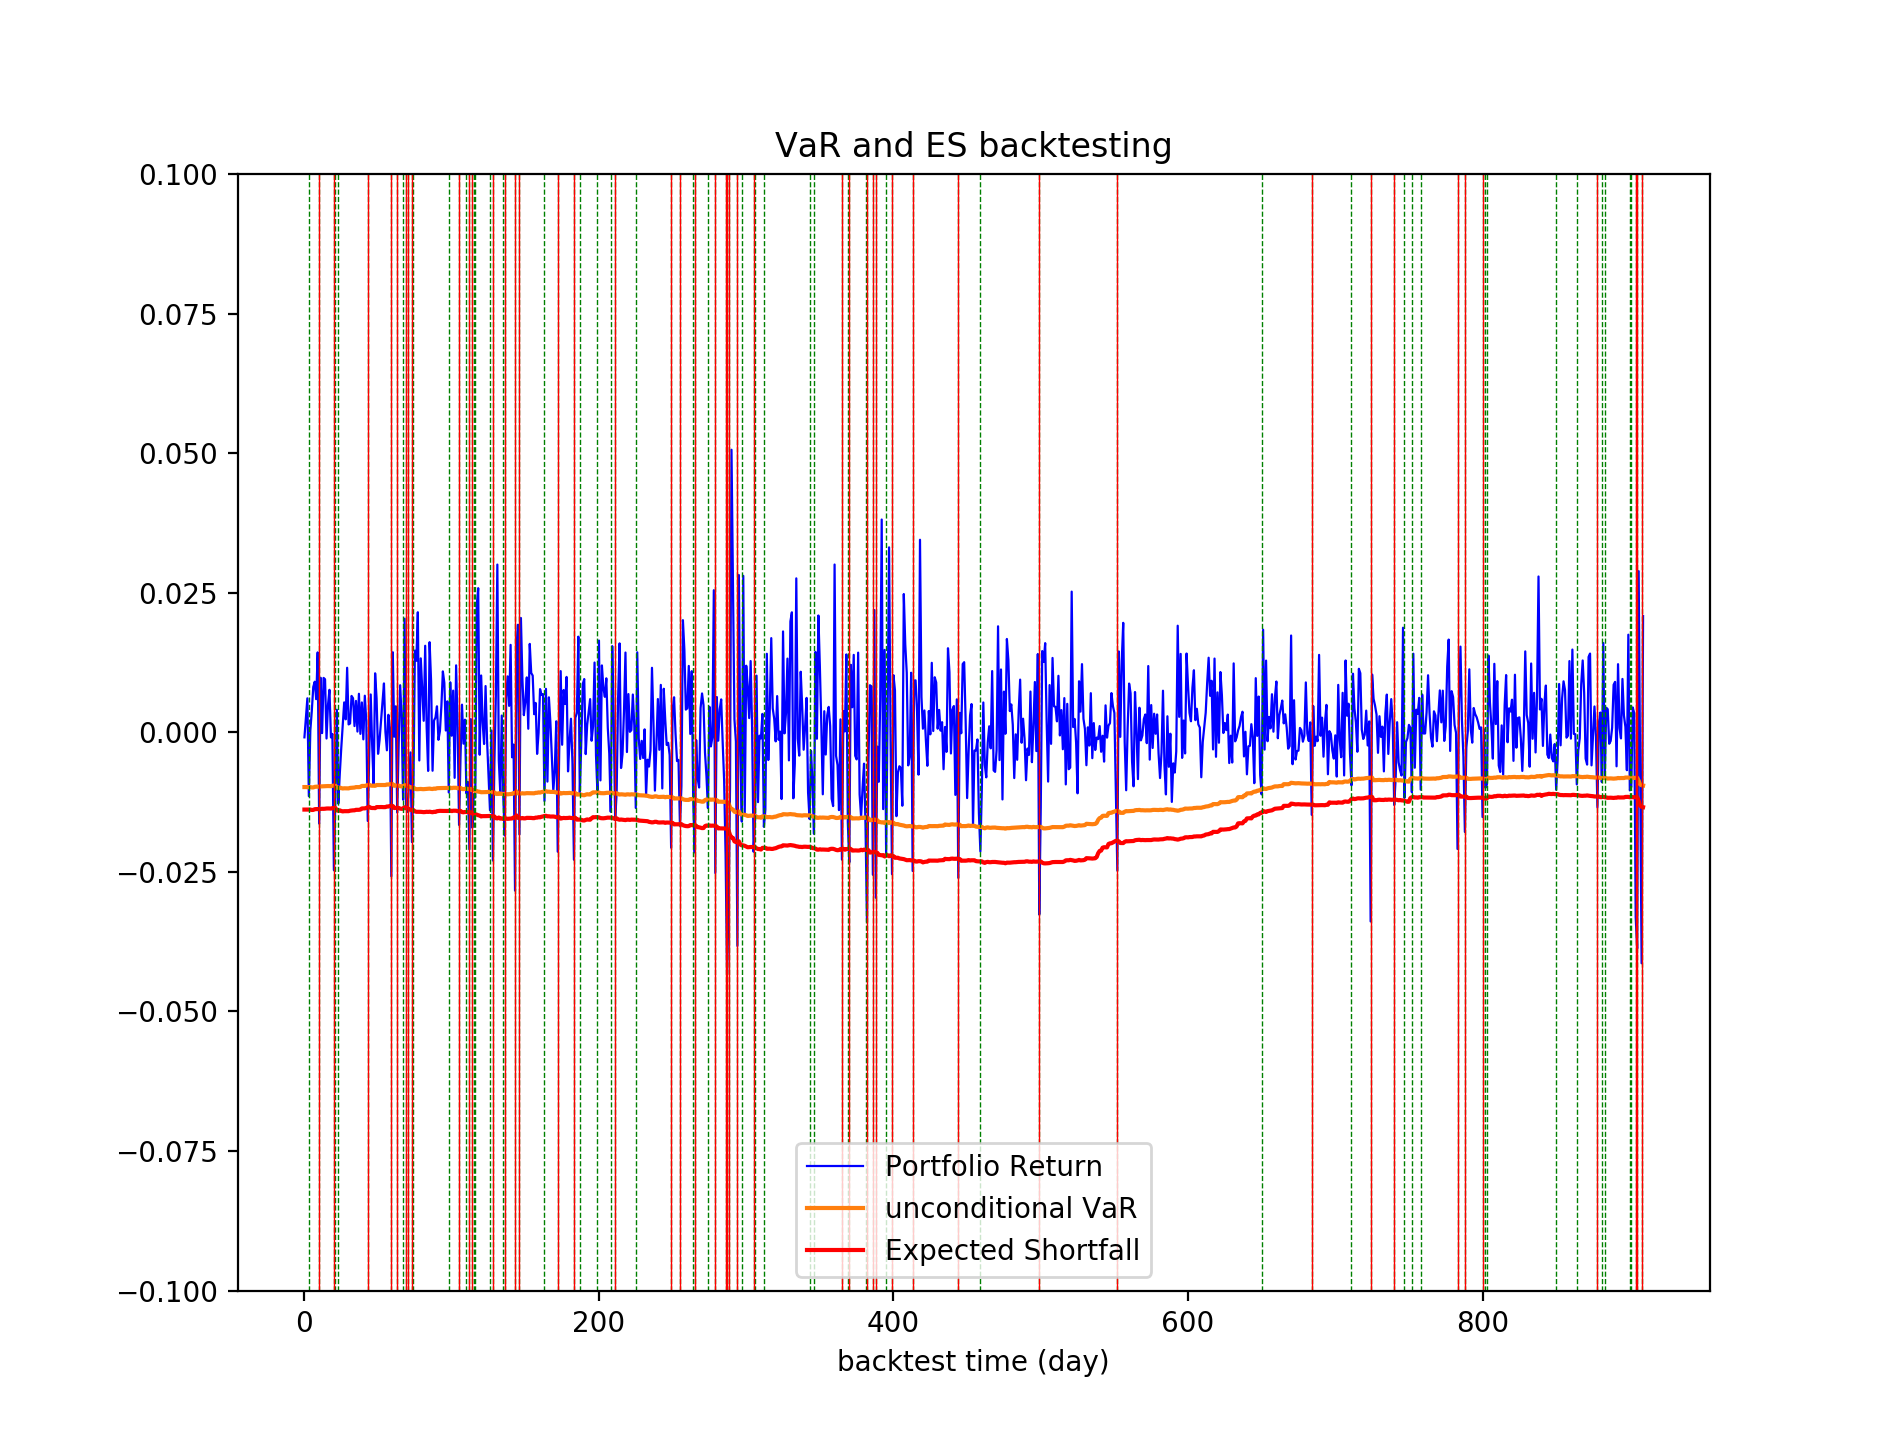
\includegraphics[scale=0.3]{Gauss_090_VaR_ES.png} &
    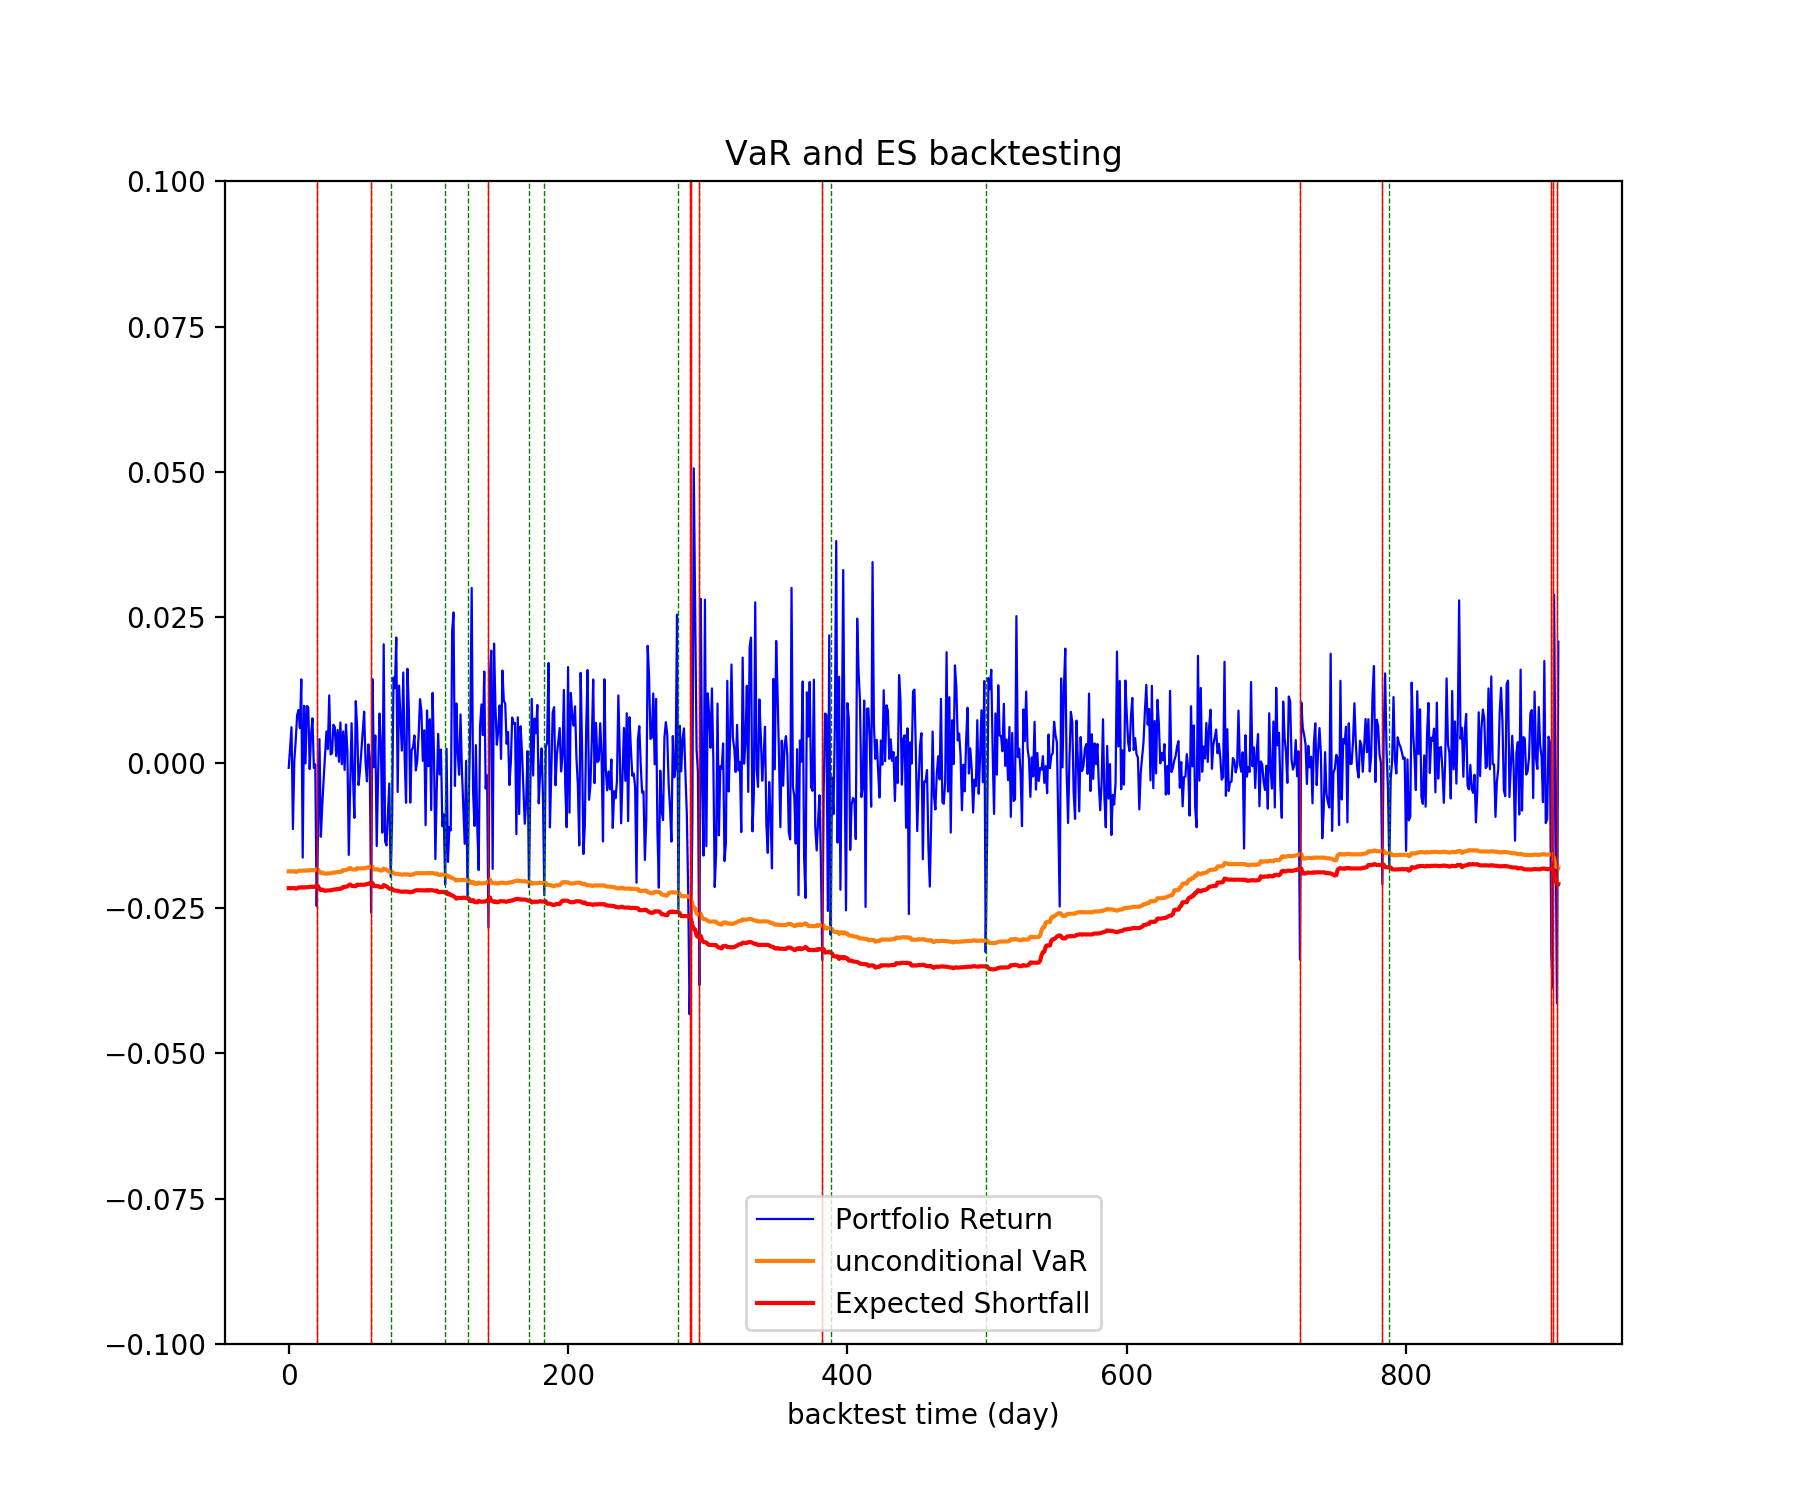
\includegraphics[scale=0.3]{Gauss_099_VaR_ES.png} \\
    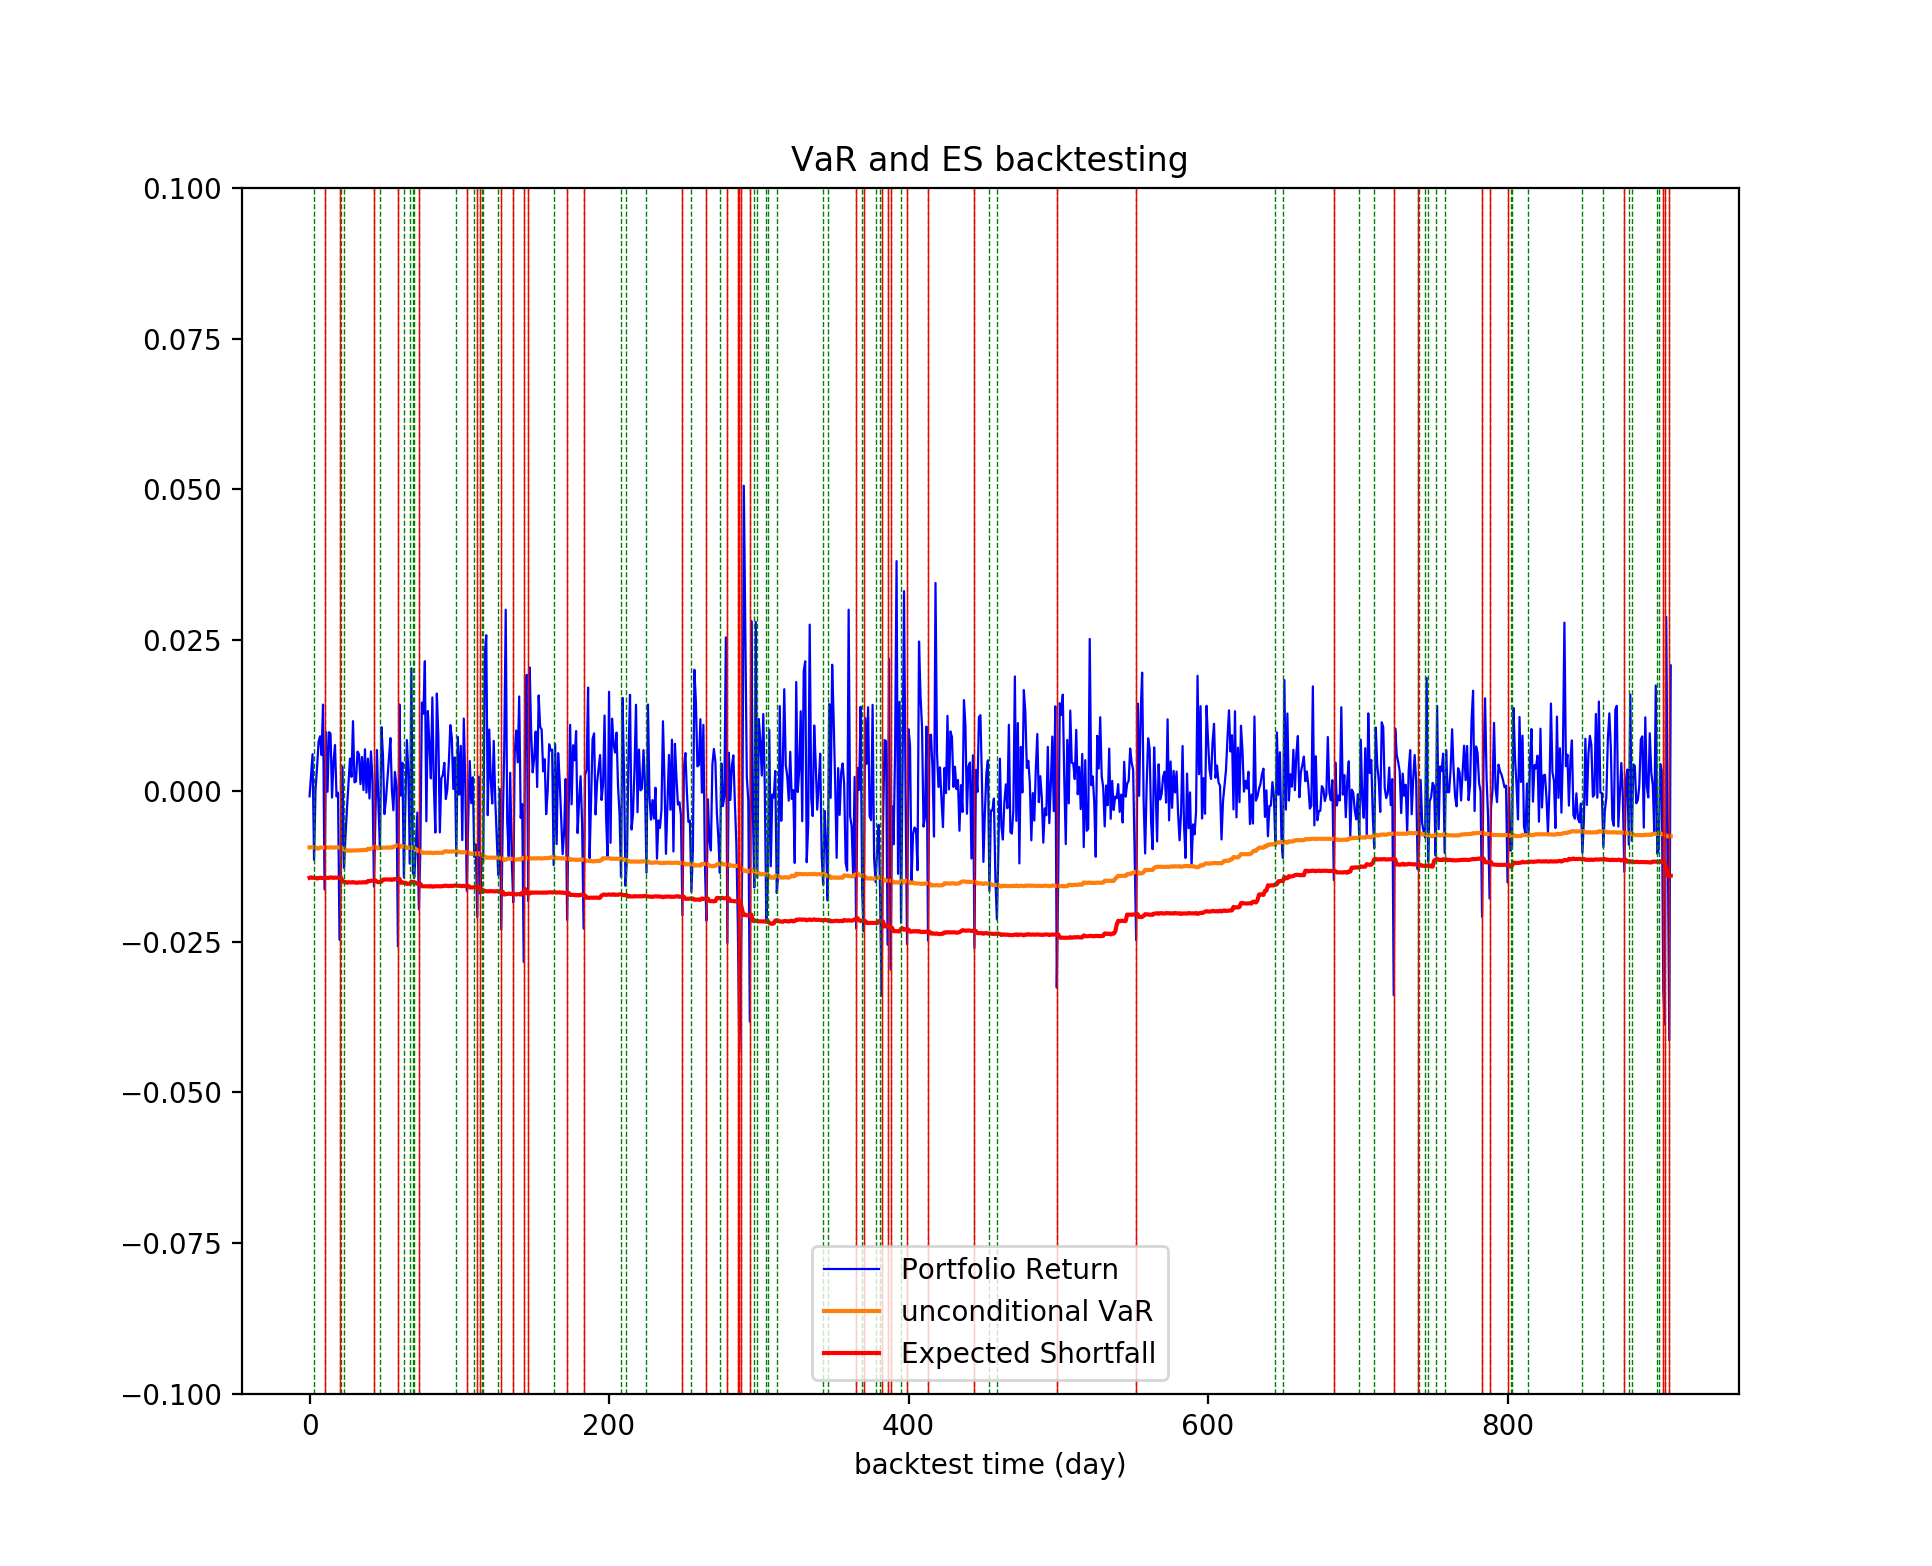
\includegraphics[scale=0.3]{HS_090_VaR_ES.png} &
    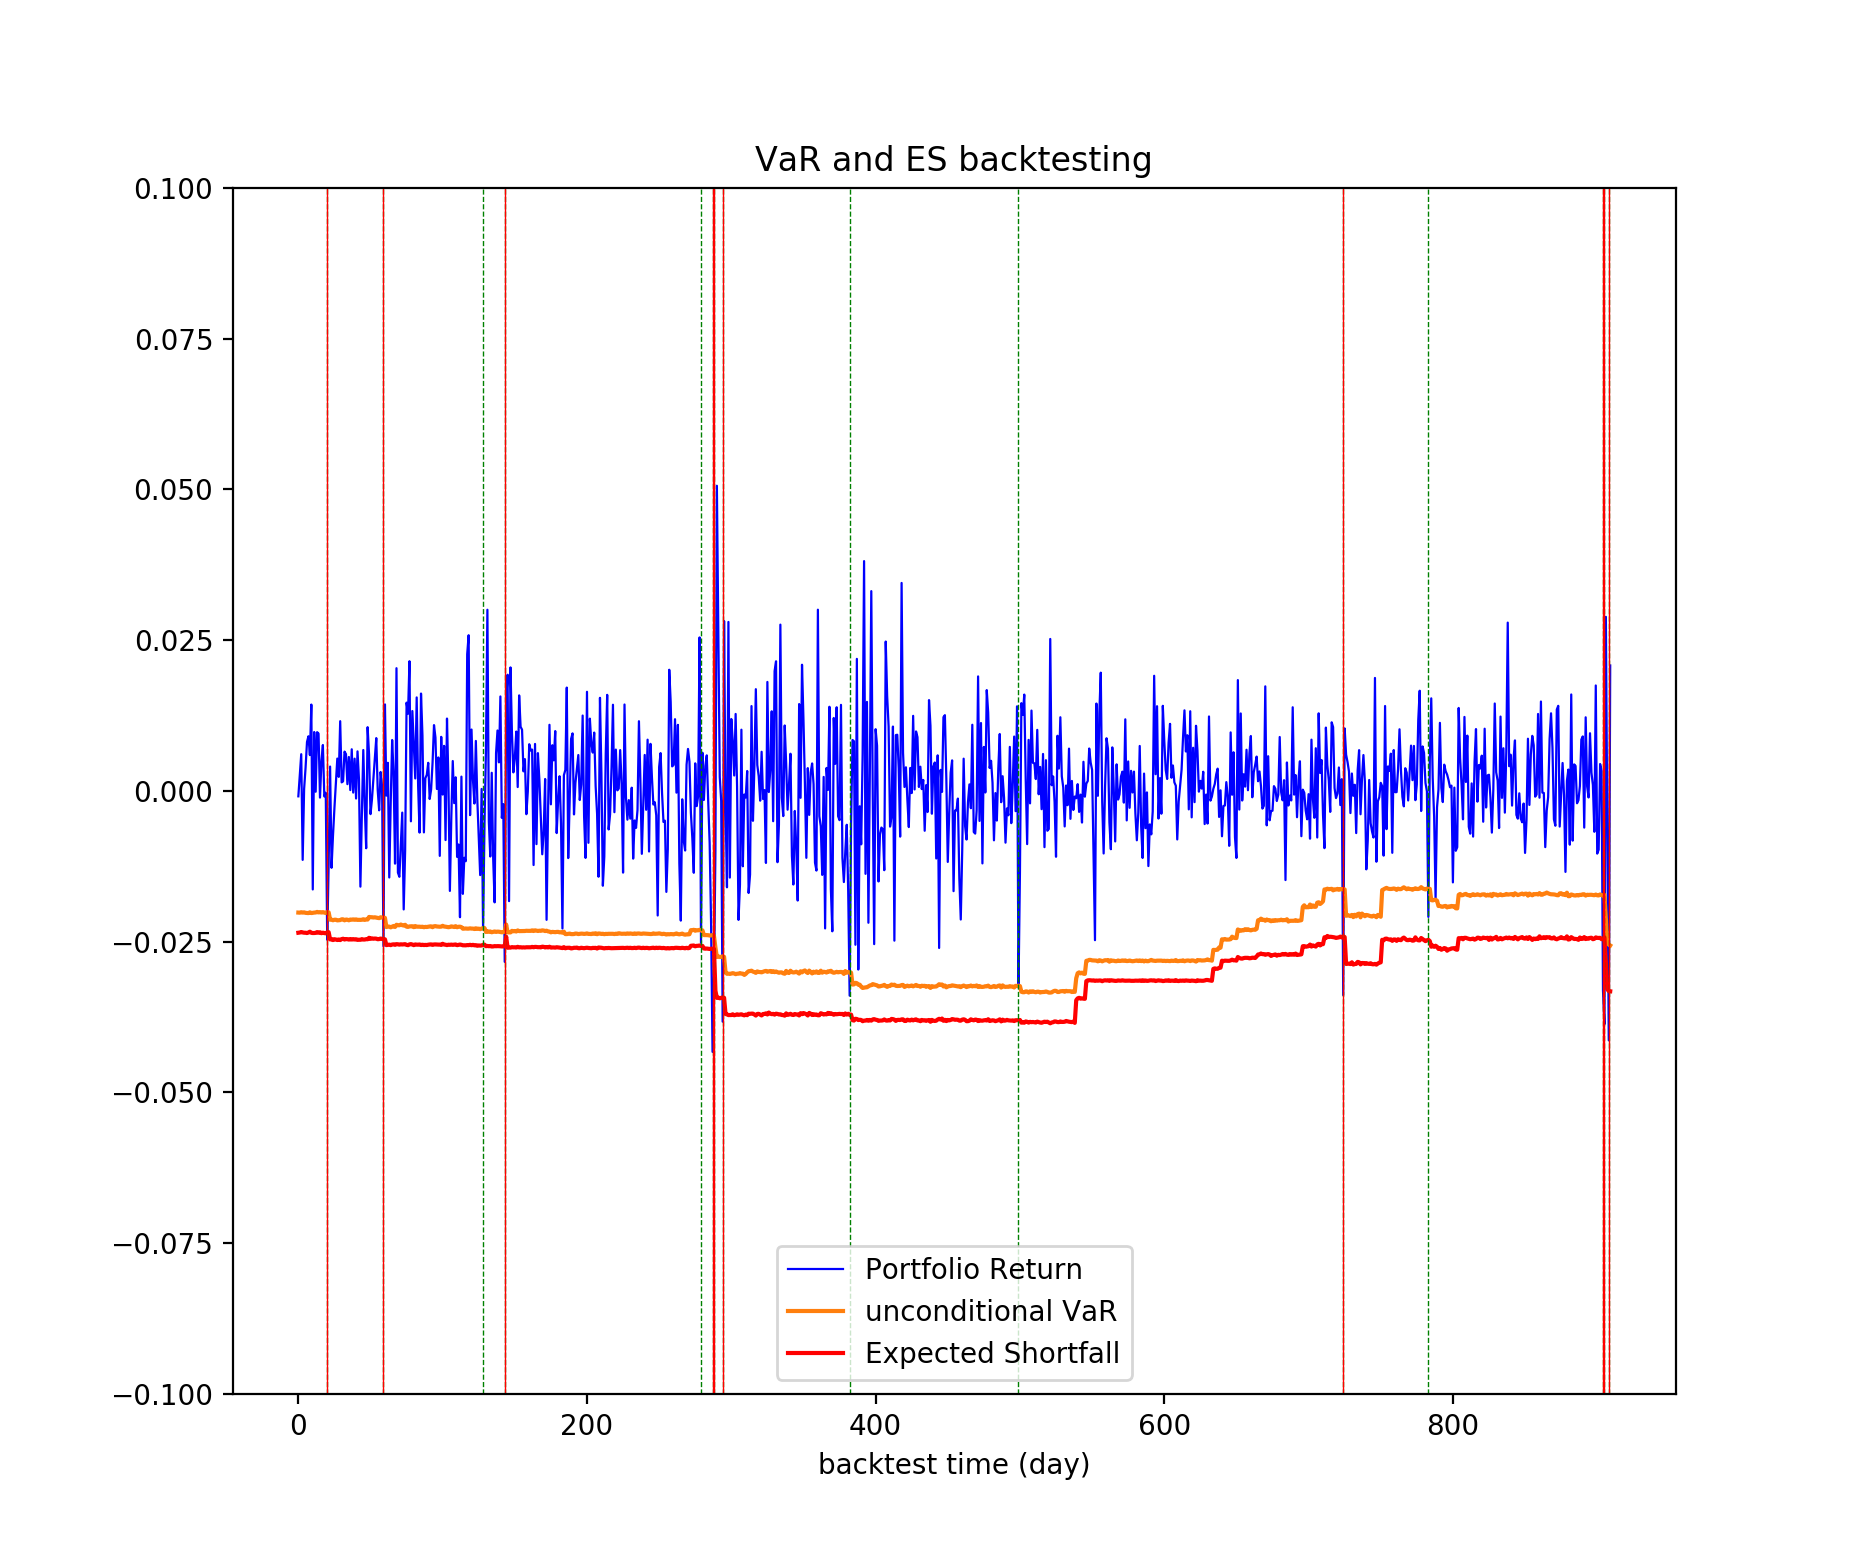
\includegraphics[scale=0.3]{HS_099_VaR_ES.png}   \\
  \end{tabular}}
  \caption{Top Left. Gaussian VaR and ES 0.90 Top Right. Gaussian VaR and ES 0.99 Bottom Left. Historical Simulation VaR and ES 0.90 Bottom Right.  Historical Simulation VaR and ES 0.99}
\end{figure}
%\subsubsection*{Kupiec Test}
\item[5.]To test if the VaR models were accurate or not in terms of number of violations or unconditional coverage, the models were examined via the Kupiec test. The Kupiec test is the log-likelihood ratio test of the model accuracy $\alpha$. If the LR does not lie below  $\chi^2_1$, we reject the null of the model is well-behaved in terms of number of hits/ violations. 
\begin{align*}
LR_{UC} &= -2ln\left(j\left(\frac{1-\alpha}{1-\hat{\alpha}} + \left(n - j\right)ln\frac{\alpha}{\hat{\alpha}}\right)\right)\\
H_0 &: LR_{UC} \sim \chi^2_1, \textsl{		good model}\\
\end{align*}
where $\alpha$ was the model confidence interval and $1 - \hat{\alpha}$ was the observed violations frequency.  $1 - \hat{\alpha}$  for our models would be $\frac{j}{1536}$ where $j$ was the total number of violations and 1536 was the rolling window times the total number of forecast. Kupiec test however is limited in testing for number of hits, not the hit sequence. If there is a cluster of hits occurred in a short-time period, the risk of the portfolio is clearly higher if the hits were scattered through a long-time period. Such that we must conducted a conditional coverage test.

%\subsubsection*{Serial dependence \& Conditional Coverage Test}
 
\item[4, 5, 6]  As explained above, we should reject the $H_0$ of a good VaR model if the hits were clustered during the backtesting. Since the events are either "hit" or "not hit", there were only four possible sequences which can be described by a first-order Markov sequence with the following transition probability matrix. 
 
 \begin{equation*}
 {\Pi_1} = \begin{bmatrix} {1-\pi_{01}} & \pi_{01} \\
  {1-\pi_{11}} & \pi_{11}  \end{bmatrix},
 \end{equation*}
 
where $\pi_{ij}$ are the conditional probabilities on the previous day event, $P\left(i|j\right)$ and $i$, $j$ are "hit" or "not hit". The likelihood function of the Markov process would be 
 \begin{equation*}
 L \left(\Pi_1\right) =  \left(1-\pi_{01}\right)^{T_{00}}  \pi_{01}^{T_{01}} \left(1-\pi_{11}\right)^{T_{10}}  \pi_{11}^{T_{11}},
 \end{equation*}
where $T_{ij}$ is the number of observations of $i$ follows by $j$. The maximal likelihood estimates of $pi_{ij}$ and $L\left( \Pi_1 \right)$ therefore are 
\begin{align*}
\hat{\pi}_{01} &= \frac{T_{01}}{T_{01}+T_{01}}\\
\hat{\pi}_{11} &= \frac{T_{11}}{T_{10}+T_{10}}\\
\hat{\Pi}_1 &= \begin{bmatrix} {1-\hat{\pi_{01}}} & \hat{\pi_{01}} \\
  {1-\hat{\pi_{11}}} & \hat{\pi_{11}}  \end{bmatrix}.
\end{align*}

Ultimately, we would like to test if $\pi_{01} = \pi_{11} = \pi$ such that the probability one violation does not depend of the previous day violation. Under the null of the hits are independently distributed , we have
\begin{align*}
 \hat{\Pi}_1 &= \begin{bmatrix} {1-\hat{\pi}} & \hat{\pi} \\
  {1-\hat{\pi}} & \hat{\pi}  \end{bmatrix}.
\end{align*}
To test the null, we use the below log-likelihood ratio test

\begin{align*}
LR_{ind} &=  -2 ln \left(\frac{L\left(\hat{\Pi}\right)}{L\left(\hat{\Pi}_1\right)}\right) \sim \chi^2_1
\end{align*}

where $L\left(\hat{\Pi}\right)$ is the $LR_{UC}$ obtained previously in the Kupiec test. To test for both if the number of violations is acceptable and the independence of the hit sequence, $H_0: \pi_{01} = \pi_{11} = p$, we test for the log-likelihood of conditional coverage $LR_{UC}$ which conveniently, by construction lies on $\chi^2_2$

\begin{align*}
LR_{CC} &= -2 ln \left(\frac{L\left( p \right)}{L\left(\hat{\Pi}_1\right)}\right) \sim \chi^2_2 \\
&= LR_{UC} + LR_{ind},
\end{align*}

Noted this test only consider the first order of the hit sequence. So it does not test for higher order dependences if they exist. 

\begin{table}[H]
\centerline{
\begin{tabular}{lllll}
\hline
                                            & Gauss        &              &              &              \\ \hline
                                            & VaR 0.90     & ES 0.90      & VaR 0.99     & ES 0.99      \\ \hline
no. of violations                           & 87           & 47           & 21           & 12           \\
$LR_{kupiec 95\%, UC}$      & 0.197962804  & 28.21570903  & 11.48030098  & 0.848518812  \\
$LR_{ind}$               & -474.8368935 & -343.1415176 & -186.191793  & -107.4456875 \\
$LR_{CC}$ & -474.6389307 & -314.9258086 & -174.711492  & -106.5971687 \\ \hline
                                            & HS Bootstrap &              &              &              \\ \hline
                                            & VaR 0.90     & ES 0.90      & VaR 0.99     & ES 0.99      \\ \hline
no. of violations                           & 91           & 41           & 15           & 10           \\
$LR_{kupiec 95\%, UC}$       & 0.0485255    & 37.61464391  & 3.231997393  & 0.08711299   \\
$LR_{ind}$               & -507.7603933 & -315.2498866 & -135.9557211 & -84.71694851 \\
$LR_{CC}$ & -507.7118678 & -277.6352426 & -132.7237237 & -84.62983552
\end{tabular}}
\end{table}

\item[7] The MRC of our portfolio was calculated as the maximum of the current 10 day $VAR_{99\%}$ or the 10 day $VAR_{99\%}$ based on the last 60 days returns.
\begin{equation*}
MRC\left(t\right) = max \left(VAR_{0.99} \left(t, t +\frac{10}{255}\right), \frac{S(t)}{60} \sum_{i=0}^{59} VAR_{0.99} \left(t-\frac{i}{255}, t - \frac{i-10}{255}\right) \right) + credit \ adjustment , 
\end{equation*}
credit adjustment was zero as we only hold stocks. However the liquidity risk and true prices were not reflected in the above formula. The MRC was 224.7775USD based on $VAR_{Gauss}$  and 248.5480USD  based on $VAR_{HS}$. 

\subsection*{10 day HS, $\mathbf{VAR_{0.99}}$ and $\mathbf{ES_{0.99}}$}
\subsubsection*{Full revaluation}
To produce the full portfolio VAR and ES, we need to calculate simulated option prices based on the simulated underlying stock prices. The Black-Scholes formula was used to calculate the options prices of \textbf{AA 140 call}, \textbf{MSFT 95 put}, \textbf{PG 85 call}. The Black-Scholes formula gives the call price and the put price as:
\begin{align*}
C_t & = S_te^{-qt}\mathcal{N}\left(d_1\right) - K e^{-rt}\mathcal{N}\left(d_2\right) \\
P_t &=  K e^{-rt} \mathcal{N} \left(-d_2\right) - S_te^{-qt}\mathcal{N}\left(-d_1\right) 
\end{align*}
where
\begin{align*}
d_1 &= \frac{ln\frac{S_t}{K} + \left(r -q +  \frac{\sigma^2}{2}\right)t}{\sigma \sqrt{t}}\\
d_2 &= d_1 - \sigma \sqrt{t}
\end{align*}
$S_t$ is the simulated stock price via Historical Simulation. 
$K$ is the strike price.
$t$ is the calender days until maturity divide by 360 of each option.
$\sigma$ is the implied annual volatility of each option given by yahoo finance. $r$ is the linear interpolated risk-free rate of each option based on the US LIBOR yield curve valued on 02/08/2018. 
\begin{align*}
r_{AAPL} = r_{2M} + (70 - 2M) * \frac{(r_{3M} - r_{2M})} { (3M - 2M)}
\end{align*}
The rates were linear interpolated between two closest quoted rates and the days to maturity demonstrated using $AAPL$ above. $q$ is the expected dividend yield. The expected  dividend yield was first derived from the Black Scholes formula based on the option price quoted on 02/09/2018. 
\begin{align*}
F_t &=C_t - P_t\\
F_t&= S_t e^{\left(r - q\right)\left(t\right)}
\end{align*}
the dividend yield was solved using the above formulas. It however gives \textbf{MSFT} and \textbf{PG} negative dividend yields. The market expected dividend yields quoted on Yahoo Finance were used instead. 
The historical returns from 01/01/2012 to 02/09/2018 of the six stocks were bootstrapped. The return dates were randomly selected with replacement $[T\times n]$ ($T=1536$ as there were 1536 historical returns available) . The $n$\footnote{n = 10 as for 10 day PnL and 10 day VaR} returns of each stocks were summed up to generate $n$ period returns which gave a $[T\times 6]$ matrix (6 as for six stocks). The simulated stock price matrix were calculated by multiplying closing prices of the stocks to the simulated returns. The three simulated option prices were calculated via Black Scholes which gave an option simulated price matrix of $[T \times 3]$. Dividing the option simulated price matrix by the option prices quoted on 02/09/2018 gave the simulated option returns. The simulated stock price matrix was combined with the simulated option price matrix, generating a $[T \times 9]$ price matrix. The 10 day simulated PnL was produced by multiplying the number of holdings in each security and dividing them by the closing prices on 02/09/2018. The 1st percentile with linear interpolation of the PnL distribution was chose to be the simulated VaR and the mean of returns which were lower than the simulated VaR was chose to be the simulated ES. The process was repeated $B$\footnote{time efficiency based $B$. as long as $B>T$} times and the means of simulated VaR and ES were the 99\%  historical simulated 10 day VaR and ES.


\subsubsection*{Delta and Gamma Approximation}

The methodology was somewhat similar with full revaluation. The differences arise from the simulating option prices. The simulated option prices were generated as follow,
\begin{align*}
C_t &= C_0 + \theta dt +  \Delta dS + \frac{1}{2} \Gamma {dS}^2
\end{align*}
where 
\begin{align*}
C_0 &: \text{call or put option price quoted on 02/09/2018}\\
dS &: S_t - S_0 \text{ , \quad simulated stock price changes}\\
\theta &: \frac{1}{T}\left(-\left(\frac{S_0 \sigma e^{-qt}}{2 \sqrt{t}}\cdot \frac{1}{\sqrt{2 \pi}}\cdot e^{\frac{-d_1^2}{2}}\right) - rKe^{-rt}\mathcal{N}\left(d_2\right) + q S_0 e^{-qt}\mathcal{N}\left(d_1 \right) \right) \text{for call}\\
&: \frac{1}{T}\left(-\left(\frac{S_0 \sigma e^{-qt}}{2 \sqrt{t}}\cdot \frac{1}{\sqrt{2 \pi}}\cdot e^{\frac{-d_1^2}{2}}\right) + rKe^{-rt}\mathcal{N}\left(-d_2\right) - q S_0 e^{-qt}\mathcal{N}\left(-d_1 \right) \right) \text{for put, where $T$ is 360 days}\\
\Delta &: e^{-qt} \mathcal{N} \left(d_1 \right) \text{for call}\\
&:  e^{-qt} \mathcal{N} \left(d_1 - 1 \right) \text{ for put}\\
\Gamma&:e^{-qt} \frac{ \phi \left(d_1\right)}{S_t \sigma \sqrt{t}} \text{,\quad $\phi$ is the normal pdf}
\end{align*}

The matrix of simulated option prices  $[T \times 3]$ were combined with the matrix of simulated stock prices $[T \times 6]$ to give the simulated price matrix  $T \times 9]$. Everything else as follow as in HS full revaluation. The simulated return matrix was generated by multiplying the number of holdings and dividing them by the closing prices on 02/09/2018. The 1st percentile was picked as simulated VaR and the mean of the lower than VaR simulated returns was took as simulated ES. The process was repeated $B$ times to generate the 99\%  historical simulated 10 day VaR and ES.

\subsubsection*{Marginal VaR and Component VaR}
To measure the sources of risk that the portfolio beared, the marginal VaR and component VaR were calculated for each security. The marginal risk was defined as the change in the portfolio risk from taking an additional dollar of in the security and the component risk is the change of portfolio risk if the security was deleted. The MVaR was calculated as the expected security returns given the portfolio return was equal to the negative VaR in the Gaussian framework. The CVaR was mutiple of the MVaR with the security weight. However, due the unlikelihood of finding portfolio return equals to the negative VaR, the condition was changed as followed 
\begin{align*}
MVaR_i \sim  & - \E \left(r_i | -VaR_\alpha \left(w\right) - \epsilon < w'r < - VaR_\alpha \left(w\right) + \epsilon \right)
\end{align*}
where $\epsilon$ was 0.005, giving a conditional tiny range. The expected security return condition to portfolio returns lower than negative VaR was estimated by averaging the sum of each simulation CVaR. The marginal expected shortfall and component expected shortfall were calculated as the expected security return condition to portfolio return which were than lower the negative expected shortfall. 
\begin{align*}
MES_i \sim  & - \E \left(r_i | w'r < - VaR_\alpha \left(w\right) \right)
\end{align*}
The mean of the conditioned security return was calculated as the $MVaR$ and $MES$ respective to the conditions. And multiplying the weights give the CVaR and CES. 
\begin{align*}
CVaR_i = w_i MVaR_i , \quad
CES_i = w_i MES_i 
\end{align*}
where 
\begin{align*}
VaR_i = \sum_{i=1}^N CVaR_i , \quad
ES_i = \sum_{i=1}^N CES_i
\end{align*}
The results are presented below. 
\begin{table}[H]
\centerline{
\begin{tabular}{lllllll}
\hline
epsilon = 0.018 &           &                 &            &           &                 &            \\ \hline
                & MVaR      & CVaR            & CVaR\_\%   & MES       & CES             & CES\_\%    \\ \hline
Sum             &           & 0.0517296335609 &            &           & 0.0732886734014 &            \\ \hline
VZ              & 0.038716  & 0.009443        & 0.18254398 & 0.057850  & 0.014110        & 0.19252548 \\
INTC            & 0.057659  & 0.007032        & 0.13593659 & 0.083749  & 0.010213        & 0.13935243 \\
JPM             & 0.060502  & 0.007378        & 0.14262517 & 0.075518  & 0.009210        & 0.12566688 \\
AAPL            & 0.062054  & 0.007568        & 0.14629809 & 0.074997  & 0.009146        & 0.12479363 \\
MSFT            & 0.050056  & 0.002442        & 0.04720665 & 0.059445  & 0.002900        & 0.03956938 \\
PG              & 0.024738  & 0.001508        & 0.02915136 & 0.027690  & 0.001688        & 0.02303211 \\
AAPL\_Opt       & 0.321727  & 0.027464        & 0.5309105  & 0.403685  & 0.034461        & 0.47020699 \\
MSFT\_Opt       & -0.263101 & -0.019251       & -0.3721438 & -0.291674 & -0.021342       & -0.2912033 \\
PG\_Opt         & 0.066796  & 0.008146        & 0.15747149 & 0.105805  & 0.012903        & 0.17605643
\end{tabular}}
\end{table}

The CVaR of each security and CES of each security should add up to VaR and ES of the portfolio respectively. However, since the MVaR, was estimated via averaging through $B \times T$ many historical simulations, there were differences between portfolio VaR and sum of CVaR. The same goes for ES. $\epsilon$ was estimated to minimize the difference between sum of CVaR and bootstrap VaR. $\epsilon$ was estimated to be . When analysising the percentage CVaR, the primary hot spot of risk contribution located on position on AAPL call option. The risk was also significantly lowered by holding MSFT put options showed in the below figure. Lowering the existing short position on apple call options and increase number of holdings of microsoft would lower overall portfolio risk.

\begin{figure}[H]
\centerline{
  \begin{tabular}{@{}cccc@{}}
    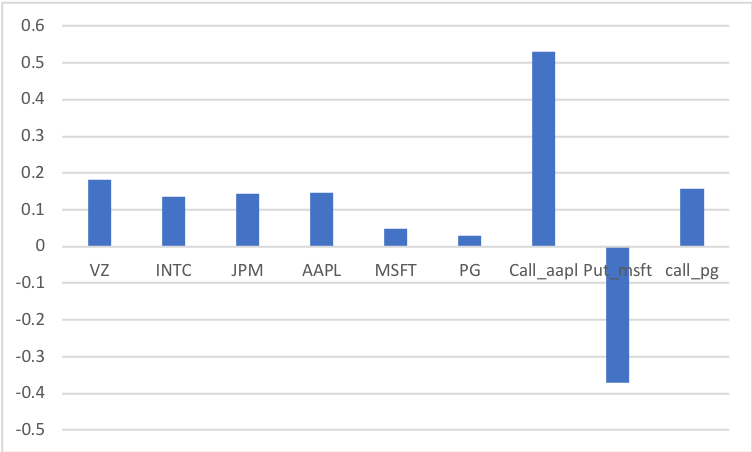
\includegraphics[scale=1.0]{HotSpot.png} \\
  \end{tabular}}
  \caption{Hot spot risk attribution of the portfolio. The blue bars are the percentage of the VaR attribution. }
\end{figure}

\subsubsection*{Best Hedge}
Additional amount of asset can be held to minimize the total portfolio risk. The idea behind this technique is to change the weight of each asset to lower the overall portfolio risk exposure. Since we have a non-parametric VaR model, the relationships between securities were not parametrised by the covariance matrix. The number of holdings of each security were added or subtracted in increments in crude simulations to obtain the minimum VaR while holding other number of securities constant. 
The function \texttt{def Best\_Hedge} in the Python script was designed to increase or decrease the number of holdings in each security, returning a VaR for each combination. The value $dw, [-10 \quad 10 \quad step: \ 0.1]$ indicates the size of the of the change, starting at -10 times. A diagonal matrix of $dw$ was first created with a dimension of $[9 \times 9]$, which represented the number of securities. The matrix was added by 1 element-wise. The new portfolio weights vector was created from multiplying the original number of holdings vector by the $nth$ column of the transformed diagonal matrix, specifying the change in the number of the specific holdings . 

\begin{align*}
\begin{bmatrix} 
dw	&	0	&	0	&	\ldots	&	0 \\
0		& 	dw&	0	&	\ldots\\
0		&	0	&	dw&	\ldots\\
\vdots		&	\vdots	&	\vdots	&	\ddots\\
0 & & & & dw \\
 \end{bmatrix} + 1 
 &\rightarrow 
 \begin{bmatrix} 
1 + dw	&	0	&	0	&	\ldots	&	0 \\
0		& 	1 + dw &	0	&	\ldots\\
0		&	0	&	1 + dw&	\ldots\\
\vdots		&	\vdots	&	\vdots	&	\ddots\\
0 & & & &1 + dw\\ 
\end{bmatrix}\\
\end{align*}
\textbf{multiply the vector of number of holdings by the nth row, when n = 0th}\\
\begin{align*}
\begin{bmatrix} 
20 \\
10 \\
10 \\
10 \\
4 \\
-5 \\
-7\\
6 \\
10\\
\end{bmatrix} \odot 
\begin{bmatrix} 
1 + dw \\
0	\\
0	\\
0	\\
0	\\
0	\\
0	\\
0 	\\
0	\\
\end{bmatrix} 
& \rightarrow 
\begin{bmatrix}
20 \times \left( 1 + dw \right) \\
10 \\
10 \\
10 \\
4 \\
-5 \\
-7\\
6 \\
10\\
\end{bmatrix}\\
\end{align*}
\textbf{the process was repeated for n = 0, 1, 2 ... 9, to create}\\
\begin{align*}
\begin{bmatrix} 
20 \times \left( 1 + dw \right) \\
10 \\
10 \\
10 \\
4 \\
-5 \\
-7\\
6 \\
10\\
\end{bmatrix} , 
\begin{bmatrix} 
20 \\
10 \times \left( 1 + dw \right) \\
10 \\
10 \\
4 \\
-5 \\
-7\\
6 \\
10\\
\end{bmatrix} , 
\begin{bmatrix} 
20 \\
10 \\
10 \times \left( 1 + dw \right) \\
10 \\
4 \\
-5 \\
-7\\
6 \\
10\\
\end{bmatrix} , \cdots 
\begin{bmatrix}[c] 
20 \\
10 \\
10  \\
10 \\
4 \\
-5 \\
-7\\
6 \\
10 \times \left( 1 + dw \right) \\
\end{bmatrix} \\
\end{align*}
\textbf{where $dw$ increases in step of 0.1 from -10 until dw reaches 10 for each nth column vector. }\\
\end{itemize}

\section{Task 6}


\end{flushleft}
\end{document}
